% -*- latex -*-
%%%%%%%%%%%%%%%%%%%%%%%%%%%%%%%%%%%%%%%%%%%%%%%%%%%%%%%%%%%%%%%%
%%%%
%%%% This TeX file is part of the course
%%%% Introduction to Scientific Programming in C++/Fortran2003
%%%% copyright 2019-2022 Victor Eijkhout eijkhout@tacc.utexas.edu
%%%%
%%%% lapack.tex : exercises for optimized linear algebra
%%%%
%%%%%%%%%%%%%%%%%%%%%%%%%%%%%%%%%%%%%%%%%%%%%%%%%%%%%%%%%%%%%%%%

Linear algebra is fundamental to much of computational science.
Applications involving \acp{PDE} come down to solving large
systems of linear equation; solid state physics involves
large eigenvalue systems.
But even outside of engineering applications linear algebra is important:
the major computational part of \ac{DL} networks involves matrix-matrix multiplications.

Linear algebra operations such as the matrix-matrix product are easy
to code in a naive way. However, this does not lead to high
performance. In these exercises you will explore the basics of a
strategy for high performance.

\Level 0 {Mathematical preliminaries}

The matrix-matrix product $C\leftarrow A\cdot B$ is defined as
\[ \forall_{ij}\colon c_{ij}\leftarrow \sum_k a_{ik}b_{kj}. \]
Straightforward code for this would be:
\begin{lstlisting}
for (i=0; i<a.m; i++)
  for (j=0; j<b.n; j++)
    s = 0;
    for (k=0; k<a.n; k++)
      s += a[i,k] * b[k,j];
    c[i,j] = s;
\end{lstlisting}
However, this is not the only way to code this operation.
The loops can be permuted, giving a total of six implementations.

\begin{exercise}
  Code one of the permuted algorithms and test its correctness. If the
  reference algorithm above can be said to be `inner-product based',
  how would you describe your variant?
\end{exercise}

Yet another implementation is based on a block partitioning. Let
$A,B,C$ be split on $2\times 2$ block form:
\[
A=
\begin{pmatrix}
  A_{11}&A_{12}\\ A_{21}&A_{22}\\
\end{pmatrix},\qquad
B=
\begin{pmatrix}
  B_{11}&B_{12}\\ B_{21}&B_{22}\\
\end{pmatrix},\qquad
C=
\begin{pmatrix}
  C_{11}&C_{12}\\ C_{21}&C_{22}\\
\end{pmatrix}
\]
Then
\begin{equation}
  \begin{array}{r@{=}l}
    C_{11}&A_{11}B_{11}+A_{12}B_{21},\\
    C_{12}&A_{11}B_{12}+A_{12}B_{22},\\
    C_{21}&A_{21}B_{11}+A_{22}B_{21},\\
    C_{22}&A_{21}B_{12}+A_{22}B_{22}\\
  \end{array}
  \label{eq:22matprod}
\end{equation}

Convince yourself that this actually computes the same product $C=A\cdot B$.
For more on block algorithms, see \HPSCref{sec:block-algebra}.

\begin{exercise}
  Write a matrix class with a multiplication routine:
\begin{lstlisting}
Matrix Matrix::MatMult( Matrix other );
\end{lstlisting}
First implement a traditional matrix-matrix multiplication,
then make it recursive.
For the recursive algorithm you need to implement
sub-matrix handling: you need to extract submatrices,
and write a submatrix back into the surrounding matrix.
\end{exercise}

\Level 0 {Matrix storage}

The simplest way to store an $M\times N$ matrix is as an array of
length~$MN$.
Inside this array we can decide to store the rows
end-to-end, or the columns.
While this decision is obviously of practical importance
for a library, from a point of performance it makes no difference.

\begin{remark}
  Historically, linear algebra software
  such as the \ac{BLAS}
  has used columnwise storage,
  meaning that the location of an element~$(i,j)$ is computed as~$i+j\cdot M$
  (we will use zero-based indexing throughout this project, both for code
  and mathematical expressions.)
  The reason for this stems from the origins of the \ac{BLAS}
  in the Fortran language, which uses column-major ordering of array elements.
  On the other hand, static arrays (such as \n{x[5][6][7]})
  in the C/C++ languages have row-major ordering,
  where element $(i,j)$ is stored in location~$j+i\cdot N$.
\end{remark}

Above, you saw the idea of block algorithms, which requires taking
submatrices. For efficiency, we don't want to copy elements into a new
array, so we want the submatrix to correspond to a subarray.

Now we have a problem: only a submatrix that consists of a sequence of
columns is contiguous. The formula $i+j\cdot M$ for location of
element $(i,j)$ is no long correct if the matrix is a subblock
of a larger matrix.

For this reason, linear algebra software describes
a submatrix by three parameters
$M,N,\mathord{LDA}$, where `LDA' stands for `leading dimension
of~$A$' (see \ac{BLAS}~\cite{Lawson:blas}, and Lapack~\cite{WN20}).
%
\begin{figure}[ht]
  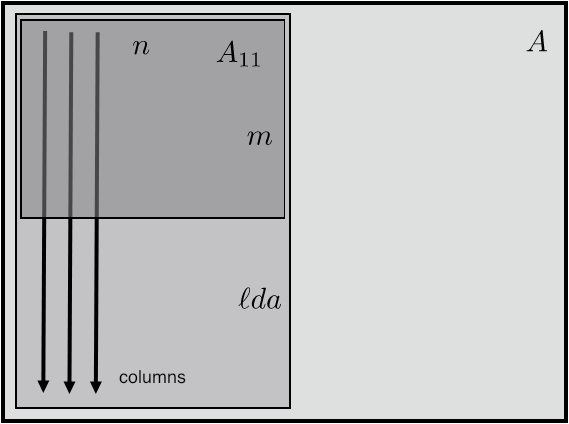
\includegraphics[scale=.5]{lapack11}
  \caption{Submatrix out of a matrix, with $M$, $N$, $\mathit{LDA}$
    of the submatrix indicated}
  \label{fig:lapack11}
\end{figure}
%
This is illustrated in figure~\textbookref{fig:lapack11}.

\begin{exercise}
  In terms of $M,N,\mathord{LDA}$, what is the location of the $(i,j)$
  element?
\end{exercise}

Implementationwise we also have a problem. If we use
\lstinline{std::vector} for storage, it is not possible to take
subarrays, since C++ insists that a vector has its own storage. The
solution is to use \indexc{span}; section~\textbookref{sec:gsl-span}.

We could have two types of matrices: top level matrices that store a
\lstinline{vector<double>}, and submatrices that store a
\lstinline{span<double>}, but that is a lot of complication.
It could be done using \lstinline{std::variant}
(section~\textbookref{sec:stl-variant}), but let's not.

Instead,
let's adopt the following idiom, where we create a vector at the top
level, and then create matrices from its memory.
%
\verbatimsnippet{spanmatrix}

(If you have not previously programmed in~C, you need to get used to
the \lstinline{double*} mechanism. 
See section~\textbookref{sec:staticarray}.)

\begin{exercise}
  Start implementing the \lstinline{Matrix} class with a constructor
\begin{lstlisting}
Matrix::Matrix(int m,int lda,int n,double *data)
\end{lstlisting}
and private data members:
%
\verbatimsnippet{matspanmembers}
%
Write a method
\begin{lstlisting}
double& Matrix::at(int i,int j);  
\end{lstlisting}
that you can use as a safe way of accessing elements.
\end{exercise}

Let's start with simple operations.
\begin{exercise}
  Write a method for adding matrices. Test it on matrices that have
  the same $M,N$, but different~$\mathord{LDA}$.
\end{exercise}

Use of the \lstinline{at} method is great for debugging, but it is not
efficient. Use the preprocessor (chapter~\textbookref{ch:cpp}) to introduce
alternatives:
\begin{lstlisting}
#ifdef DEBUG
  c.at(i,j) += a.at(i,k) * b.at(k,j)
#else
  cdata[ /* expression with i,j */ ] += adata[ ... ] * bdata[ ... ]
#endif
\end{lstlisting}
where you access the data directly with
%
\verbatimsnippet{matspandata}

\begin{exercise}
  Implement this. Use a cpp \indexpragma{define} macro for the
  optimized indexing expression. (See section~\textbookref{sec:cpp-define-fun}.)
\end{exercise}

\Level 1 {Submatrices}

Next we need to support constructing actual submatrices. Since we will
mostly aim for decomposition in $2\times2$ block form, it is enough to
write four methods:
\begin{lstlisting}
Matrix Left(int j);
Matrix Right(int j);
Matrix Top(int i);
Matrix Bot(int i);
\end{lstlisting}
where, for instance, \lstinline{Left(5)} gives the columns with~$j<5$.

\begin{exercise}
  Implement these methods and test them.
\end{exercise}

\Level 0 {Multiplication}

You can now write a first multiplication routine, for instance with a prototype
\begin{lstlisting}
void Matrix::MatMult( Matrix& other,Matrix& out );
\end{lstlisting}

Alternatively, you could write
\begin{lstlisting}
Matrix Matrix::MatMult( Matrix& other );
\end{lstlisting}
but we want to keep the amount of creation/destruction of objects to a minimum.

\Level 1 {One level of blocking}

Next, write
\begin{lstlisting}
void Matrix::BlockedMatMult( Matrix& other,Matrix& out );
\end{lstlisting}
which uses the $2\times2$ form above.

\Level 1 {Recursive blocking}

The final step is to make the blocking recursive.

\begin{exercise}
  Write a method
\begin{lstlisting}
void RecursiveMatMult( Matrix& other,Matrix& out );
\end{lstlisting}
  which 
  \begin{itemize}
  \item Executes the $2\times2$ block product, using again
    \lstinline{RecursiveMatMult} for the blocks.
  \item When the block is small enough, use the regular
    \lstinline{MatMult} product.
  \end{itemize}
\end{exercise}

\Level 0 {Performance issues}

If you experiment a little with the cutoff between the regular and
recursive matrix-matrix product, you see that you can get good factor
of performance improvement. Why is this?

The matrix-matrix product is a basic operation in scientific
computations, and much effort has been put into optimizing it. One
interesting fact is that it is just about the most optimizable
operation under the sum. The reason for this is, in a nutshell, that
it involves $O(N^3)$ operations on $O(N^2)$ data. This means that, in
principle each element fetched will be used multiple times, thereby
overcoming the \indextermbus{memory}{bottleneck}.

To understand performance issues relating to hardware, you need to do some
reading. Section~\HPSCref{sec:cache} explains the crucial
concept of a \indexterm{cache}.

\begin{exercise}
  Argue that the naive matrix-matrix
  product implementation is unlikely actually to reuse data.

  Explain why the recursive strategy does lead to data reuse.
\end{exercise}

Above, you set a cutoff point for when to switch from the recursive to
the regular product.

\begin{exercise}
  Argue that continuing to recurse will not have much benefit once the
  product is contained in the cache. What are the cache sizes of your
  processor?

  Do experiments with various cutoff points. Can you relate this to
  the cache sizes?
\end{exercise}

\Level 1 {Parallelism (optional)}

The four clauses of equation~\textbookref{eq:22matprod} target independent
areas in the $C$ matrix, so they could be executed in parallel on any
processor that has at least four cores.

Explore the OpenMP library to parallelize the \lstinline{BlockedMatMult}.

\Level 1 {Comparison (optional)}

The final question is: how close are you getting to the best possible
speed? Unfortunately you are still a way off. You can explore that as
follows.

Your computer is likely to have an optimized implementation,
accessible through:
\begin{lstlisting}
#include <cblas.h>

cblas_dgemm
  ( CblasColMajor, CblasNoTrans, CblasNoTrans,
    m,other.n,n, alpha,adata,lda,
    bdata,other.lda,
    beta,cdata,out.lda);
\end{lstlisting}
which computes $C\leftarrow \alpha A\cdot B+\beta C$.

\begin{exercise}
  Use another cpp conditional to implement \lstinline{MatMult} through
  a call to \indextermtt{cblas_dgemm}. What performance do you now get?
\end{exercise}

You see that your recursive implementation is faster than the naive
one, but not nearly as fast as the CBlas one. This is because
\begin{itemize}
\item the CBlas implementation is probably based on an entirely
  different strategy~\cite{GotoGeijn:2008:Anatomy}, and
\item it probably involves a certain amount of assembly coding.
\end{itemize}

